% !TEX root = main.tex
%\myparagraph{Key points}
%\begin{enumerate}[1.]
%%	\item	Session $\pi$ calculus with process passing. DONE
%%	\item	Identify session $\pi$ and process passing subcalculi and their polyadic variants. DONE
%%	\item	Bisimulation theory for higher-order session semantics. DONE
%%	\item	New triggered bisimulation, related to J\&R's. DONE
%%	\item   Elementary values key to characterizations of behavioral equivalence. DONE
%	\item	Types provide techniques to prove completeness without matching. \jp{TBD}
%	\item	We are interested in encodings with properties a la Gorla. 
%                We extended them to typed setting. \jp{TBD}
%%	\item	Encode name-passing to pure process abstraction calculus, with name abstractions. DONE
%%	\item	Type of the recursion encoding uses non tail recursive type $\trec{t}{\btinp{t} \tinact}$. DONE
%%	\item	Encode higher-order semantics to first order semantics. DONE
%%	\item	Negative result. Cannot encode shared names using only shared names.
%%	\item   Extensions with higher-order abstractions and polyadicity also explored. DONE
%\end{enumerate}

%\smallskip 
%
%\myparagraph{Important things to explain}
%Explain our \HO is very small without containg name passing 
%\[ 
%\abs{x}.P \quad \appl{x}{u}
%\]

%Explain we input only characteristic processes.  
%
%\[
%\lambda x.\mapchar{S}{x}
%\]

%\subsection{Higher-Order Session Calculi}
\noi 
By combining features from the $\lambda$-calculus and the $\pi$-calculus, 
in \emph{higher-order process calculi} exchanged values may contain  processes. 
In this paper, we consider higher-order calculi with \emph{session primitives},
thus enabling the specification of reciprocal exchanges (protocols) 
for higher-order mobile processes, 
which can be verified via type-checking using \emph{session types}~\cite{honda.vasconcelos.kubo:language-primitives}.
%These calculi allow us to specify   
%session protocols in which higher-order values 
%(mobile code) can be exchanged in a type-safe manner. 
%; 
%governed by session types, 
%such protocols cleanly distinguish between 
%linear and unrestricted behaviors in 
%%directed %point-to-point 
%communications.
The study of higher-order concurrency has received significant attention, 
from typed and untyped perspectives.
%in particular via  comparisons with the first-order mobility of the $\pi$-calculus~\cite{MilnerR:calmp1}. 
Although models of session-typed 
communications with features of higher-order concurrency exist~\cite{tlca07,DBLP:journals/jfp/GayV10},
their  \emph{tractable behavioral equivalences} and \emph{relative expressiveness}
remain little understood. 
%for higher-order session calculi. 
%these two issues 
%have been throughly studied
%%are well-understood 
%for higher-order languages without sessions \cite{},
%but not for higher-order process calculi with sessions.
%This is unfortunate, given the wide applicability of session-based concurrency; indeed,
%session types are expressive enough to describe complex 
%communication structures found in practical protocols,  expressible, e.g., via recursive session types.
%Clarifying the status of typed equivalences and relative expressiveness for session languages
Clarifying their status is not only useful for, 
e.g.~justifying non-trivial mobile protocol
optimisations, but also for transferring key reasoning techniques
between (higher-order) session calculi. Our discovery 
is that linearity of session types plays a vital role to 
offer new equalities and fully abstract encodability, not proposed before.   

The main higher-order language in our work, denoted \HOp,
extends the higher-order $\pi$-calculus~\cite{SangiorgiD:expmpa} with session primitives:
it contains constructs for 
%session establishment
synchronisation on shared names, 
recursion, 
name abstractions (i.e., functions from name identifiers $x$ to processes, $\lambda x.P$) and applications $(\lambda x.P)a$;
and session communication (value passing and
labeled choice using linear names). 
We present two significant subcalculi of \HOp, restrict to higher- and first-order mobility:
the \HO-calculus, which is \HOp without recursion and name passing, and 
the (session) \sessp-calculus, which is \HOp without abstractions and applications.  
While the \sessp-calculus is 
in essence the calculus in~\cite{honda.vasconcelos.kubo:language-primitives}, 
this paper shows that \HO  is a new core calculus 
for higher-order session concurrency.

In the first part of the paper, we address tractable behavioral equivalences
for \HOp.
A well-studied behavioral equivalence in the higher-order setting 
is \emph{context bisimilarity}~\cite{San96H},
a labelled characterisation of barbed congruence, 
which offers an appropriate discriminative power at the price of heavy universal quantifications in output clauses.
Obtaining alternative characterisations 
is thus a recurring issue 
in the study of higher-order calculi. 
Our approach 
shows the protocol specifications given by session types are 
important to  limit 
the behavior of higher-order session processes. 
Exploiting elementary processes inhabiting session types, 
this limitation is formally enforced by 
a refined (typed) labelled transition system (LTS)
that narrows down the spectrum of allowed process behaviors, 
thus enabling tractable reasoning techniques. 
Two tractable characterisations of bisimilarity 
are shown to coincide with contextual bisimilarity.

We then move on to 
%in the second part of the paper we 
assess the expressivity 
 of \HOp, \HO, and \sessp as delineated by typing. 
We establish strong correspondences between 
these calculi  via type-preserving, fully abstract encodings up to 
behavioural equalities. While it is well-known that the higher-order 
$\pi$-calculus is encodable into the $\pi$-calculus, our main result is 
encoding \HOp into \HO where name-passing is absent.  

We demonstrate the essence of encoding name passing into \HO: 
to encode name output, we ``pack''
the name to be passed around into a suitable abstraction; 
upon reception, the receiver must ``unpack'' this object following a precise protocol; an encoding in \HO is given as:
\[
\begin{array}{rcll}
  \map{\bout{a}{b} P}	&=&	\bout{a}{ \abs{z}{\,\binp{z}{x} (\appl{x}{b})} } \map{P} \\
  \map{\binp{a}{x} Q}	&=&	\binp{a}{y} \newsp{s}{\appl{y}{s} \Par \bout{\dual{s}}{\abs{x}{\map{Q}}} \inact}
\end{array}
\]
where $a,b$ are names; $s$ and $\dual{s}$ are 
dual session end-points;
%$\lambda x.P$ is a name abstraction of $P$; $\appl{x}{a}$ is a name application; 
$\bout{a}{V} P$ and 
$\binp{a}{x} P$ denote an input and output at $a$;   
and $\newsp{s}P$ is hiding. 
A (deterministic) reduction between session endpoints 
($s$ and $\dual{s}$) gurantees to correctly unpack name $a$.

We further extend our encodability results to 
\HOp with \emph{higher-order} abstractions (denoted by \HOpp) 
and \HOp with the polyadic name passing and abstraction (\pHOp); and 
their super-calculus  (\PHOpp) (which is equivalent to \cite{tlca07}). 
%Here again the usage information given by session types is essential to define encodings
%and to state their semantic correspondences.
% Building upon established notions for (untyped) processes~(e.g.,~\cite{DBLP:journals/iandc/Gorla10}), 
% we
%define a notion of \emph{precise encoding} that 
%requires the translation of both process and types, and 
%focuses on process mappings that preserve (session) typing. 
%Thus, our encodings only relate source and target 
%processes 
%with  
%proper communication structures (given by session types).
A further result shows that 
shared names
%as required in the session establishment phase,
strictly add expressive power 
to session calculi. 
Fig.~\ref{fig:express} summarises %our expressivity 
these results. %including the three extensions of \HOp. 

\begin{figure}[t]
%ADD~FIGURE!
	\begin{center}
		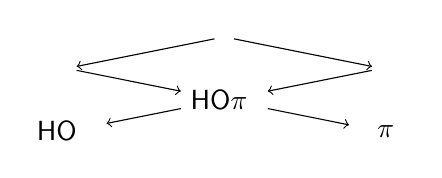
\begin{tikzpicture}
			\node	(PHOpp)	at	(0, 0.8)		{\PHOpp};
			\node	(HOpp)	at	(-2, 0.4)	{\HOpp};
			\node	(PHOp)	at	(2, 0.4)	{\PHOp};
			\node	(HOp)	at	(0, 0)		{$\mathsf{HO}{\pi}^{~}$};
			\node	(HO)	at	(-2, -0.4)	{$\mathsf{HO}{~}^{~}$};
			\node	(sessp)	at	(2, -0.4)	{$~~\pi^{~}$};

			\draw[->]	(PHOpp) -- (HOpp);	%(0, 1.25) -- (-2, 1);
			\draw[->]	(PHOpp) -- (PHOp);	%(0, 1.25) -- (2, 1);

			\draw[->]	(HOpp) -- (HOp);	%(2, 0.5) -- (0, 0.25);
			\draw[->]	(PHOp) -- (HOp);	%(-2, 0.5) -- (0, 0.25);

			\draw[->]	(HOp) -- (HO);		%(0, -0.25) -- (-2, -0.5);
			\draw[->]	(HOp) -- (sessp);	%(0, -0.25) -- (2, -0.5);


			% Polyadic HO and Polyadic pi
	%		\node	at	(-3, 0)		{\PHO};
	%		\node	at	(3, 0)		{\Psessp};

	%		\draw[->]	(0, 1.5) -- (-3, 0.25);
	%		\draw[->]	(0, 1.5) -- (3, 0.25);

	%		\draw[->]	(3, -0.25) -- (2, -0.5);
	%		\draw[->]	(-3, -0.25) -- (-2, -0.5);




		\end{tikzpicture}
	\end{center}
\caption{Summary of Expressiveness Results. \label{fig:express}}
\Hline
\end{figure}

\smallskip

\myparagraph{Outline.}
\S\,\ref{sec:overview} overviews the key idea of our tractable bisimulations.
\noi \S\,\ref{sec:calculus} presents the calculi; 
\S\,\ref{sec:types} presents types.
The tractable bisimulations are in \S\,\ref{sec:behavioural}.
The notion of encoding is in \S\,\ref{s:expr} and
\S\,\ref{sec:positive} %and \S\,\ref{sec:negative}
presents expressiveness results.
%present positive and negative encodability results, resp;
In \S\,\ref{sec:extension} we discuss extensions; 
\S\,\ref{sec:relwork} concludes with related works.
An appendix summarises the typing system. 
The paper is self-contained. 
{\bf\em Omitted definitions, additional related work, and  proofs 
%can be found
are 
in~\cite{KouzapasPY15}.} 

